\documentclass{article}
\usepackage[utf8]{inputenc}
\usepackage{enumitem}
\usepackage{tikz-cd}
\usepackage{amsmath}
\usepackage{amssymb}
\usepackage{calc}

\newcounter{artCounter}
\setcounter{artCounter}{0}
\newcounter{maxArts}
\setcounter{maxArts}{0}

\newcommand{\showLastArt}{\csname artsDef\romannumeral\the\numexpr\arabic{maxArts} - 1\relax\endcsname}

\newcommand{\showArt}{
\csname artsDef\roman{artCounter}\endcsname
\addtocounter{artCounter}{1}
\ifnum \value{artCounter}=\value{maxArts}
\setcounter{artCounter}{0}
\fi
}

\newcommand{\registerArt}[1]{%
\expandafter\newcommand\csname artsDef\roman{maxArts}\endcsname{#1}%
\addtocounter{maxArts}{1}%
}

\title{Notto - Category for the Working Mathematician}
\author{tkunn}
\date{August 2020}

\begin{document}

\registerArt{{
$$ \langle \wedge \ \_\  \wedge \rangle $$
}}

\registerArt{{
$$ \langle Q\ _\perp\ Q \rangle $$
}}

\registerArt{{
$$ \langle Q\ _{^{\dot{\smile}}}\ Q \rangle $$
}}

\registerArt{{
\begin{center}
\begin{tikzcd}[ampersand replacement=\&]
\& *\arrow[ld]\arrow[rd,"h"] \& \& \& *\arrow[ld,swap,"i"]\arrow[rd] \& \\
* \& \& * \& * \& \& * \\
\\
\\
\& \& \phi \arrow[r] \& \theta \& \&
\end{tikzcd}
\end{center}
}}

\registerArt{{
\begin{center}
\begin{tikzcd}[ampersand replacement=\&]
\& *\arrow[ld]\arrow[rd,"h"] \& \& \& *\arrow[ld,swap,"i"]\arrow[rd] \& \\
* \& \& * \& * \& \& * \\
\\
\\
\& \& \phi \arrow[r, bend right=20] \& \theta \& \&
\end{tikzcd}
\end{center}
}}

\registerArt{{
\begin{center}
\begin{tikzcd}[sep=2em,ampersand replacement=\&]
\& *\arrow[ld]\arrow[rd,"h"] \& \& \& \& *\arrow[ld,swap,"i"]\arrow[rd] \& \\
* \& \& * \& \& * \& \& * \\
\\
\\
\& \& \& \phi \arrow[r, loop] \& \& \&
\end{tikzcd}
\end{center}
}}

\registerArt{{
\begin{center}
\begin{tikzcd}[sep=2em,ampersand replacement=\&]
\arrow[dddd, bend right=30]   \pi\& \& *\arrow[ld]\arrow[rd,"h"] \& \& \& \& *\arrow[ld,swap,"i"]\arrow[rd] \& \& \mathcal{H} \arrow[loop right, distance=5em] \arrow[llllllll, dashrightarrow, bend right=25]\\
\& * \& \& * \& \& * \& \& * \&\\
\\
\\
\arrow[rrrrrrrr, dashrightarrow, bend right=20] \theta\& \& \& \& \phi \arrow[r, loop] \& \& \& \& \mathcal{P} \arrow[uuuu, bend right=30]
\end{tikzcd}
\end{center}
}}

\registerArt{{
\begin{center}
\begin{tikzcd}[ampersand replacement=\&]
\& *\arrow[ld]\arrow[rd,"h"] \& \& \& *\arrow[ld,swap,"i"]\arrow[rd] \& \\
* \& \& * \& * \& \& * \\
\\
\& \phi \arrow[rrr,bend right=50] \& \& \& \theta \&
\end{tikzcd}
\end{center}
}}

\registerArt{{
\begin{center}
\begin{tikzcd}[row sep=3em,column sep=3em,ampersand replacement=\&]
\&\&Sa^\prime\arrow[dddd,shorten=21mm,xshift=8mm,yshift=8mm]\arrow[dddd,shorten=21mm,xshift=-8mm,yshift=8mm]\\
\&\&\&\\
Sa\arrow[rrrr,shorten=5em,yshift=1.5mm,leftrightarrow,bend right]\arrow[rruu]\&\&\upsilon\&\&Ta^\prime\arrow[lluu]\\
\&\&\&\&\\
\&\&Ta\arrow[rruu]\arrow[lluu]
\end{tikzcd}
\end{center}
}}

\registerArt{{
\begin{center}
\begin{tikzpicture}
\node at (-1em,0) {(}; 
\node at (1em,0) {)}; 
\node at (0,0) {$\cdot\tau\cdot$}; 
\node[scale=0.5] at (0,-0.5em) {\smile}; 
\end{tikzpicture}
\end{center}
}}

\registerArt{{
\begin{center}
\begin{tikzpicture}
\node at (-1em,0) {(}; 
\node at (1em,0) {)}; 
\node at (0,0) {$\cdot\tau\cdot$}; 
\node[scale=0.5] at (0,-0.5em) {\frown}; 
\end{tikzpicture}
\end{center}
}}

\registerArt{{
\begin{center}
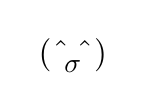
\begin{tikzpicture}
\node[scale=1.2] at (-1em,-0.1em) {(}; 
\node[scale=1.2] at (1em,-0.1em) {)}; 
\node[scale=1.3] at (0,0) {$\hat{}$\ \ $\hat{}$}; 
\node at (0,-0.5em) {$\sigma$}; 
\end{tikzpicture}
\end{center}
}}

\registerArt{{
\begin{center}
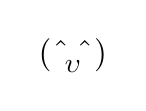
\begin{tikzpicture}
\node[scale=1.2] at (-1em,-0.1em) {(}; 
\node[scale=1.2] at (1em,-0.1em) {)}; 
\node[scale=1.3] at (0,0) {$\hat{}$\ \ $\hat{}$}; 
\node at (0,-0.5em) {$\upsilon$}; 
\end{tikzpicture}
\end{center}
}}

\registerArt{{
\begin{center}
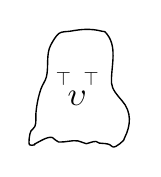
\begin{tikzpicture}
\draw  [xshift=-55,yshift=25,yscale=-0.007,xscale=0.007, color={rgb, 255:red, 0; green, 0; blue, 0 }][line width=0.5] [line join = round][line cap = round] (198,243.5) .. controls (205.86,239.93) and (222.32,228.44) .. (231,231.5) .. controls (235.28,233.01) and (237.48,239.09) .. (242,239.5) .. controls (253.39,240.54) and (266.56,235.76) .. (277,237.5) .. controls (278.29,237.71) and (289.76,241.75) .. (292,242.5) .. controls (293.63,243.04) and (304.42,237.94) .. (310,238.5) .. controls (311.48,238.65) and (314.49,241.28) .. (316,241.5) .. controls (322.04,242.36) and (329.71,241.86) .. (335,244.5) .. controls (338.75,246.37) and (339.71,250.8) .. (346,247.5) .. controls (351.26,244.75) and (355.67,240.56) .. (360,236.5) .. controls (361.31,235.27) and (361.2,233.11) .. (362,231.5) .. controls (373.16,209.17) and (374.98,185.05) .. (357,164.5) .. controls (350.07,156.58) and (338.44,143.93) .. (338,132.5) .. controls (336.8,101.3) and (350.85,64.35) .. (326,39.5) .. controls (324.05,37.55) and (322.52,39.13) .. (320,38.5) .. controls (299.88,33.47) and (283.38,34.98) .. (264,38.5) .. controls (257.75,39.64) and (248.37,38.66) .. (243,42.5) .. controls (236.85,46.89) and (230.44,59) .. (228,63.5) .. controls (218.94,80.22) and (224.47,103.63) .. (220,121.5) .. controls (218.09,129.14) and (212.58,135.75) .. (210,143.5) .. controls (205.3,157.61) and (202.3,171.91) .. (201,187.5) .. controls (200.36,195.13) and (202.08,204.3) .. (199,211.5) .. controls (198.03,213.77) and (192.81,218.36) .. (192,219.5) .. controls (189.31,223.27) and (187.29,242.27) .. (189,244.5) .. controls (191.03,247.14) and (195.67,244.5) .. (199,244.5) ;
\node[scale=0.7] at (0,0) {$\top$\ \ $\top$}; 
\node[scale=1.2] at (0,-0.7em) {$\upsilon$}; 
\end{tikzpicture}
\end{center}
}}

\maketitle

This is solutions for problems on the second edition of \textit{Category for the Working Mathematician} by S. Mac Lane.

\section{}

\subsection{}

\subsection{}

\subsection{}

\subsubsection{}



\subsubsection{}



\subsubsection{}



\subsubsection{}



\subsubsection{}



\subsection{}

\subsubsection{}



\subsubsection{}



\subsubsection{}



\subsubsection{}



\subsubsection{}



\subsubsection{}



\subsection{}

\subsubsection{}



\subsubsection{}



\subsubsection{}



\subsubsection{}



\subsubsection{}



\subsubsection{}



\subsubsection{}



\subsubsection{}



\subsubsection{}



\subsection{}

Let $U$ be a set that satisfies following conditions:

\begin{enumerate}[label=(\roman*)]
\item $x \in u \in U \Rightarrow x \in U$
\item $(u \in U \wedge v \in U) \Rightarrow (\{u, v\}, \langle u, v \rangle, u \times v \in U)$
\item \begin{enumerate}[label=(\arabic*)]
\item $x \in U \Rightarrow \mathcal{P} x \in U$
\item $x \in U \Rightarrow \bigcup x \in U$
\end{enumerate}
\item $\omega \in U$, where $\omega = \{0,1,2,\dots\}$ is a set of all finite ordinal numbers.
\item If there exists a surjection $f : a \rightarrow b$ and $a \in U$ and $b \subset U$, then $b \in U$.
\end{enumerate}

\subsubsection{}

\showArt

For all $q \in \prod_i f_i$, we can construct a bijection $r : I \rightarrow q$. $q \subset U$ because $\forall w \in q,\ \exists j \in I,\ w \in f_j \in U$. Since $I \in U$ and $q \subset U$, we can say $q \in U$. Therefore $\prod_i f_i \subset U$.

Let $|f_k| \geq |f_i|$ for all $i$. Then, we can construct a surjection $g : f_k^I \rightarrow \prod_i f_i$. Also, we can construct a surjection $h : X \rightarrow f_k^I$, with X is either $\mathcal{P} f_k$ or $\mathcal{P} I$. As $X \in U$, $g \circ h : X \rightarrow \prod_i f_i$ and $\prod_i f_i \subset U$, we can say $\prod_i f_i \in U$.

\subsubsection{}



\showArt

\begin{enumerate}[label=(\alph*)]
\item We can construct a bijection $g :  I \rightarrow \{f_i\ |\ i \in I\}$, $g(i) = f_i$. As $I \in U$ and $f_i \in U$ for all $i$, $\{f_i\ |\ i \in I\} \in U$. Therefore $ \bigcup_i f_i = \bigcup \{f_i\ |\ i \in I\} \in U$.
\item Because $x \in U$, we have $y \in U$ for all $y \in x$. Therefore we can apply $f : x \rightarrow x, f(i) = i$ to (a) to get $\bigcup x \in U$.

Because $a \in U$ and $b \subset U$, we can apply $f$ to (a) to get $\bigcup_i f_i \in U$. $f$ is surjective, therefore $b = \bigcup_i f_i$. Hence $b \in U$.
\end{enumerate}

\subsection{}

\subsection{}

\section{}

\subsection{}

\subsection{}

\subsection{}

\subsubsection{}



\showArt

In this section, $\times_S$ is a product operation for sets, $\times_C$ is for categories, $\times_G$ is for groups and $\times_M$ is for monoids.

\textit{Monoids.} Let $M, N$ be a monoid with object $m, n$ respectively. The only object in $M \times_C N$ is $\langle m, n \rangle$. ... (TODO)

\textit{Groups.} Let $G, H$ be a group with object $a, b$ respectively. $G \times_C H$ ... (TODO)

\textit{Sets.} Let $A, B$ be discrete categories. The set of all objects in $A \times_C B$ is $X = A \times_S B$. The set of all arrows in $A \times_C B$ is $\{\langle f, g \rangle\ |\ a \in A,\ b \in B,\ f \in A(a, a)\ \wedge\ g \in B(b, b)\} = \{\langle \mathrm{id}_A(c_0), \mathrm{id}_B(c_1) \rangle\ |\ c \in X\}$. Therefore  $A \times_C B$ is a discrete category of $X = A \times_S B$.

\subsubsection{}



\showArt

Let P, Q be preorders. $\forall a \forall b\ | \hom(a, b) | \leq 1$ for both P and Q. Therefore, for all $p_1 \in P$, $p_2 \in P$, $q_1 \in Q$, $q_2 \in Q$, $| \hom_{P \times Q}(\langle p_1, q_1 \rangle, \langle p_2, q_2 \rangle) | = | \hom_P(p_1, p_2) \times \hom_Q(q_1, q_2) | \leq 1$. Hence $P \times Q$ is preorder.

\subsubsection{}



\showArt

Let $\mathrm{id}_X(a) : a \rightarrow a$ be identity in category $X$.

Let the set of all object in $C$ be the product set $\prod_i C_i$ and $C(a, b) = \prod_i C_i(a_i, b_i)$. Let $\mathrm{id}_C(c)_i = \mathrm{id}_{C_i}(c_i)$ for all $c \in C$. Now, we prove $C$ has a universal property:

\begin{enumerate}
\item For every $i$ there is a functor $P_i : C \rightarrow C_i$.
\item For every category $B$ such that a functor $G_i : B \rightarrow C_i$ presents for every $C_i$, there is a functor $F : B \rightarrow C$, which makes the following diagram commute.

\begin{center}
\begin{tikzcd}[sep=4em]
B \arrow[d, swap, "F", dashrightarrow] \arrow[dr, "G_i"] \\
C \arrow[r, "P_i"] & C_i
\end{tikzcd}
\end{center}
\end{enumerate}

First, we prove $P_i : C \rightarrow C_i$ exists. Let the object function be $P_i(x) = x_i$. Let the arrow function be $P_i(f) = f_i$. For all object $c \in C$, $P_i(\mathrm{id}_C(c)) = \mathrm{id}_C(c)_i = \mathrm{id}_{C_i}(c_i) = \mathrm{id}_{C_i}(P_i(c))$. For all arrow $f$, $g$ in C, $P_i(g \circ f) = (g \circ f)_i = g_i \circ f_i =  P_i(g) \circ P_i(f)$. Therefore $P_i$ is a functor.

Second, we prove $F : B \rightarrow C$ exists. Let the object function be $F(x)_i = G_i(x)$. Let the arrow function be $F(f)_i = G_i(f)$. For all object $b \in B$, $F(\mathrm{id}_B(b))_i = G_i(\mathrm{id}_B(b)) =  \mathrm{id}_{C_i}(G_i(b)) = \mathrm{id}_{C_i}(F(b)_i)$. Thus $F(\mathrm{id}_B(b)) = \mathrm{id}_{C}(F(b))$. For all arrow $f$, $g$ in B, $F(f \circ g)_i = G_i(f \circ g) = G_i(f) \circ G_i(g)$. Thus $F(f \circ g) = F(f) \circ F(g)$. Therefore $F$ is a functor.

\subsubsection{}



\showArt

In $\mathbf{Matr}_K$, the object set is all positive integers $\{1, 2, 3, ...\} = \omega \setminus \{0\}$. $\mathbf{Matr}_K(n, m)$ is all rectangular matrix on $K$ of shape $m \times n$. Therefore $\mathbf{Matr}_K^{\mathrm{op}}$ has the same objects $\omega \setminus \{0\}$ and  $\mathbf{Matr}_K^{\mathrm{op}}(n, m)$ is all rectangular matrix on $K$ of shape $n \times m$.

\subsubsection{}



\showArt

Let $R_T \subseteq (T \rightarrow \mathbb{R})$ be a ring whose elements are continuous functions from a topological space $T$ to real number. We construct $R_T$ as follows:

\begin{enumerate}
    \item Additive identity. $0_{R_T} : x \mapsto 0$.
    \item Multiplicative identity. $1_{R_T} : x \mapsto 1$.
    \item Addition. $f + g : x \mapsto f(x) + g(x)$.
    \item Multiplication. $f \times g : x \mapsto f(x) \times g(x)$.
\end{enumerate}

Let $X$ and $Y$ be any topological spaces. If we have a continuous function $f : Y \rightarrow X$, we can construct a ring homomorphism $H(f) = h : R_X \rightarrow R_Y$. We define $h(r) = r \circ f$. Then $h(0_{R_X}) = 0_{R_Y}$, $h(1_{R_X}) = 1_{R_Y}$, $(h(s + t))(x) = (s + t)(f(x)) = s(f(x)) + t(f(x))$, $(h(s \times t))(x) = (s \times t)(f(x)) = s(f(x)) \times t(f(x))$. Therefore $H(f)$ is a ring homomorphism.

Now we construct a functor $F : \mathbf{Top}^{\mathrm{op}} \rightarrow \mathbf{Rng}$. Let the object function be $F(A) = R_A$ and the arrow function be $F(g) = H(g^{\mathrm{op}})$. For all arrow $a, b$ in $\mathbf{Top}^{\mathrm{op}}$, $F(b \circ a) = H((b \circ a)^{\mathrm{op}}) = H(a^{\mathrm{op}} \circ b^{\mathrm{op}}) = H(b^{\mathrm{op}}) \circ H(a^{\mathrm{op}}) = F(b) \circ F(a)$. For all topological space $T \in \mathbf{Top}^{\mathrm{op}}$, $F(\mathrm{id}(T)) = H(\mathrm{id}(T)) = \mathrm{id}(R_T)$. Therefore $F$ is a functor and $\overline{F}$ is a contravariant functor on $\mathbf{Top}$ to $\mathbf{Rng}$.

\subsection{}

\subsubsection{}















\subsubsection{}



\showArt

For any functor $T : X \rightarrow B$, if its object function is $T(a) = b$, its arrow function maps $\mathrm{id}(a)$ to $\mathrm{id}(b)$. Such a functor $T$ is an object of $B^X$.

Let $R, S : X \rightarrow B$ be functors and $\tau$ be a map on an object of X to an arrow in $B$. $(\tau : R\ \dot{\rightarrow}\ S) \Leftrightarrow (\forall x \in X,\ \tau_x(R(x)) = S(x))$. Therefore $\hom(R, S) = \{\tau\ |\ \forall x \in X,\ \tau_x(R(x)) = S(x)\}$. Therefore an arrow on $R$ to $S$ exists iff $(\forall x, y \in X,\ e_R(x, y) \rightarrow e_S(x, y))\ \wedge\ (\forall x \in X,\ \hom(R(x), S(x)) \neq \emptyset)$, where $e_T(x, y) \Leftrightarrow (\exists a \in B, \{x, y\} \subseteq \{ w\ |\ a = T(w) \})$.

\subsubsection{}



\showArt

An object of $\mathbf{Ab}^{\mathbf{N}}$ is a map on $\mathbb{N}$ to $\mathbf{Ab}$. Same as above, $\hom(R, S) = \{\tau\ |\ \forall n \in N,\ \tau_n(R(n)) = S(n)\}$. In other words, a map $\tau : \mathbb{N} \rightarrow (\mathbf{Ab} \rightarrow \mathbf{Ab})$ is an arrow iff, for every $n \in \mathbb{N}$, there is a corresponding group homomorphism $\tau_n$ on $R(n)$ to $S(n)$, and, for every $m \in \mathbb{N}$ such that $R(n) = R(m)$, $S(n) = S(m)$. 

\subsubsection{}



\showArt

Let $R, S : P \rightarrow Q$. Then $R$ and $S$ are objects of $Q^P$. Let $\tau$ be a natural transform $\tau : R\ \dot{\rightarrow}\ S$. $\tau$ is an arrow on $R$ to $S$ in $Q^P$. Since $\tau$ is natural and $P$ is preorder, the following diagram commutes for every pair of objects $p, p^\prime \in P$. $a = f(p,\,p^\prime)$, where $f(p, p^\prime)$ is the only arrow on $p$ to $p^\prime$. Since $Q$ is preorder, $\tau p = g(Rp, Sp)$, where $g(Rp, Sp)$ is the only arrow on $Rp$ to $Sp$.

\begin{center}
\begin{tikzcd}
Rp \arrow[d, swap, "{Ra}"] \arrow[r, "{\tau p}"] & Sp \arrow[d, "{Sa}"]\\
Rp^\prime \arrow[r, "{\tau p^\prime}"] & Sp^\prime
\end{tikzcd}
\end{center}

From the two downward arrows in the diagram, we can say that $\mathrm{Im}(R)$ and $\mathrm{Im}(S)$ contain the preorder structure of $P$. There are two functors $P \rightarrow \mathrm{Im}(R)$ and $P \rightarrow \mathrm{Im}(S)$, where $\mathrm{Im}(T)$ is a category from the image of the object function of $T$ and all arrows between any two pairs in the image.

As explained above, $\sigma p = g(Rp, Sp)$ for all $\sigma : R\ \dot{\rightarrow}\ S$. Thus $|\hom(R, S)| \leq |\{\sigma\ |\ \forall p \in P,\ \sigma p = g(Rp, Sp)\}| = 1$. Therefore $Q^P$ is preorder.

\subsubsection{}



\showArt

Let $\mathbf{Fin}$ be a category of all finite sets. The object is every finite set and the arrow is every mapping between every pair of finite sets.

Let $G$ be a finite group. $G$ is a category of only one object. Every arrow $a$ in $G$ has its inverse $a^{-1}$ such that $a \circ a^{-1} = a^{-1} \circ a = \mathrm{id}$.

$\mathbf{Fin}^G$ is a category that have any functor on $G$ to $\mathbf{Fin}$ as objects and any natural transform between two objects as arrows. The group $G$ has only one object $x \in G$, thus any functor $T \in \mathbf{Fin}^G$ map $x$ to a finite set $T(x) \in \mathbf{Fin}$, and endomorphisms of $x$ to endomorphisms of $T(x)$. For any arrow $a$, $b$ in $G$, $T(b \circ a) = T(b) \circ T(a)$. Also, $\mathrm{id} = T(\mathrm{id}) = T(a \circ a^{-1}) = T(a) \circ T(a^{-1})$. Thus any element in the image of the arrow function of $T$ is invertible. Therefore $T$ is a permutation representation of $G$.

Now, let $\tau : R\ \dot{\rightarrow}\ S$ be an arrow in $\mathbf{Fin}^G$. Then, the following diagram commutes for any arrow $a$ in $G$:
\begin{center}
\begin{tikzcd}
Rx \arrow[d, swap, "Ra"] \arrow[r, "\tau x"] & Sx \arrow[d, "Sa"]\\
Rx \arrow[r, "\tau x"] & Sx
\end{tikzcd}
\end{center}
From the diagram, $\hom(R, S) = \{\tau\ |\ \forall a,\ \tau x \circ R a = S a \circ \tau x\}$... what does it mean???? TODO

\subsubsection{}

\subsubsection{}

\subsubsection{}

\subsection{}

\subsubsection{}

\showArt

symbols: A B C F S T

We prove there is a bijection $F : \mathbf{Cat}(A \times B, C) \rightarrow \mathbf{Cat}(A, C^B)$.

Let $FT = S$, where $T : A \times B \rightarrow C$ and $S : A \rightarrow C^B$. First, we make the object function of $S$. Given $a \in A$, we make a subcategory $A_a \subseteq A$, a category of an object $a$ and an arrow $\mathrm{id}(a)$. Trivially, there is a functor $f_a : B \rightarrow A_a \times B$ ($f_a(b) = \langle a, b \rangle$ for objects, $f_a(b) = \langle \mathrm{id}(a), b \rangle$ for arrows). As $A_a \times B \subseteq A \times B$, now we define $Sa : B \rightarrow C$ as $Sa = T \circ f_a$. Second, we make the arrow function of $S$. Let $Sa = \tau$, where $a : a_0 \rightarrow a_1$ is an arrow in $A$, $\tau : S a_0\ \dot{\rightarrow}\ S a_1$, $\tau b = T\langle a, \mathrm{id}(b) \rangle$. Let $g : b_0 \rightarrow b_1$ be an arrow in $B$. Then $Sa_1g(\tau b_0(Sa_0b_0)) = Sa_1b_1 = \tau b_1(Sa_0g (Sa_0b_0))$. Thus $\tau$ is natural.

Next, we prove that for all $S : A \rightarrow C^B$, there exists $T : A \times B \rightarrow C$, such that $FT = S$. First, we prove it for the object function of $T$. Let $a \in A$, $b \in B$, $T\langle a, b \rangle = Sab$. $FTab = T\langle a, b \rangle$, thus $FT = S$. Second, we prove it for the arrow function. Let there be two arrows $a$ in $A$ and $b$ in $B$, and $T\langle a, b \rangle = Sa(\mathrm{dom}(b))$. Then $FTab = Sab$, thus $FT = S$.

Finally, we prove that for all $T_0,\ T_1 : A \times B \rightarrow C$, if $FT_0 = FT_1$, then $T_0 = T_1$. Let $FT_0 = FT_1$ and $n \in \{0,\ 1\}$. We write $T_=\langle x, y \rangle$ when $T_0\langle x, y \rangle = T_1\langle x, y \rangle$. First, for all $a \in A$, $b \in B$, $FT_nab = T_n\langle a, b \rangle$. Thus $T_=\langle a, b \rangle$ (for objects). Second, for every object $a \in A$, arrow $b$ in $B$, $FT_nab = T_n\langle \mathrm{id}(a), b \rangle$, and, for every arrow $a$ in $A$, object $b \in B$, $FT_nab = T_n\langle a, \mathrm{id}(b) \rangle$. Now, let $a : a_0 \rightarrow a_1$ be any arrow in $A$ and $b : b_0 \rightarrow b_1$ be any arrow in $B$. $T_=\langle \mathrm{id}(a_0), b \rangle$ and $T_=\langle a, \mathrm{id}(b_1)\rangle$, thus $T_=(\langle \mathrm{id}(a_0), b \rangle \circ \langle a, \mathrm{id}(b_1) \rangle)$. Hence $T_=\langle a, b \rangle$ (for arrows).

\subsubsection{}

\showArt

For any $x \in (A \times B)^C$, there are two functions $G(c) = x(c)_0$ and $H(c) = x(c)_1$. Let the object function be $F(x) = \langle G, H \rangle$, where $F : (A \times B)^C \rightarrow A^C \times B^C$.

For any natural transform $\tau : (A \times B)\ \dot{\rightarrow}\ C$, there are two natural transforms $\tau_0 : A\ \dot{\rightarrow}\ C$ and $\tau_1 : B\ \dot{\rightarrow}\ C$. Let $\tau_0(x) = $ and $\tau_1(x) = $.

Thus we can construct the arrow function $F(\tau) = \langle \tau_0, \tau_1 \rangle$.

Let $L_0, L_1 : X \rightarrow (T \downarrow S)$ be two functors which makes the diagram commute.

TODO

\subsubsection{}

\subsubsection{}

\subsubsection{}

\subsubsection{}

\subsubsection{}

\subsubsection{}

\subsection{}

\subsubsection{}

\showArt

(seems to be trivial...)

In $\mathbf{CRng}$, $f : K \rightarrow L$ is a ring homomorphism on $K$ to $L$. Thus $K \downarrow \mathbf{CRng}$ is the category of all small commutative $K$-algebra.

\subsubsection{}

\showArt

(seems to be trivial...)

We make a functor $F : C \rightarrow (C \downarrow t)$. Since $t$ is a terminal object in $C$, for all object $c \in C$, there is a unique arrow $a_c : c \rightarrow t$. We use the arrow-making function $a_c$ as the object function of $F$. For any objects $c_0, c_1 \in C$, $|C(c_0, c_1)| = |(C \downarrow t)(a_{c_0}, a_{c_1})|$. Since $a_c$ is a bijection, both the object and arrow function of $F$ is bijective. Thus $C$ is isomorphic to $(C \downarrow t)$. 

\subsubsection{}

\showArt

An alternative diagram for objects:

\begin{center}
\begin{tikzcd}
  &    & t \arrow[mapsto, d, "t_2"]\arrow[mapsto, dll, swap, "t_0"]\arrow[mapsto, drr, "t_1"] \\
e \arrow[mapsto, r, swap, "Te"] & Te & \arrow[mapsto, l, "\mathrm{dom}f"] f \arrow[mapsto, r, swap, "\mathrm{cod}f"] & Sd & \arrow[mapsto, l, "Sd"] d 
\end{tikzcd}
\end{center}

A diagram for arrows:

\begin{center}
    \begin{tikzcd}
      & &
\langle k, h \rangle
     \arrow[mapsto, d]\arrow[mapsto, dll, swap]\arrow[mapsto, drr] & &\\
    k \arrow[mapsto, r, swap] & Tk & \arrow[mapsto, l]\langle Tk, Sh \rangle\arrow[mapsto, r, swap] & Sh & \arrow[mapsto, l] h
    \end{tikzcd}
\end{center}

An alternative diagram for arrows:

\begin{center}
    \begin{tikzcd}
      &    & t \arrow[mapsto, d, "\langle Tt_0{,} St_1 \rangle"]\arrow[mapsto, dll, swap, "t_0"]\arrow[mapsto, drr, "t_1"] \\
    k \arrow[mapsto, r, swap, "Tk"] & Tk & \arrow[mapsto, l, "t^\prime_0"] t^\prime \arrow[mapsto, r, swap, "t^\prime_1"] & Sh & \arrow[mapsto, l, "Sh"] h
    \end{tikzcd}
\end{center}

\subsubsection{}

\showArt

Let $T, S : D \rightarrow C$ be functors, $\tau : T\ \dot{\rightarrow}\ S$ be a natural transform, $\tau^\prime : D \rightarrow (T \downarrow S)$ be a functor such that $(\tau_d)_0 = (\tau_d)_1 = d$. Thus the object function maps an object $d \in D$ to $\langle d, d, Td \rightarrow Sd \rangle$. Then, for any arrow $g : d \rightarrow d^\prime$ in $D$, $f : Td \rightarrow Sd$ and $f^\prime : Td^\prime \rightarrow Sd^\prime$ in $C$, the following diagram commutes:

\begin{center}
    \begin{tikzcd}
    Td \arrow[r, "f"] \arrow[d, "Tg"] & Sd \arrow[d, "Sg"]\\
    Td^\prime \arrow[r, "f^\prime"] & Sd^\prime
    \end{tikzcd}
\end{center}

This means that $\tau^\prime$ is a natural transform on $T$ to $S$.

\subsubsection{}

\showArt

Let $E$, $C$, $D$, $X$ be categories, $P$, $Q$, $R$, $P^\prime$, $Q^\prime$, $R^\prime$, $T$, $S$ be functors. We prove that if the following diagram commutes, there is a unique functor $L : X \rightarrow (T \downarrow S)$ that keeps it commute.

\begin{center}
    \begin{tikzcd}[row sep=4em, column sep=4em]
      & & X \arrow[dashed, bend right, swap]{dd}[near start]{L}
     \arrow[d, "Q^\prime"]\arrow[dll, swap, "P^\prime"]\arrow[drr, "R^\prime"] & &\\
    E \arrow[r, "T"] & C & \arrow[l]C^2\arrow[r, swap] & C & \arrow[l, swap, "S"] D\\
    & & (T \downarrow S)\arrow[u, swap, "Q"]\arrow[ull, "P"]\arrow[urr, "R", swap]
    \end{tikzcd}
\end{center}

For any object $x \in X$, let $e^\prime = P^\prime x$, $d^\prime = R^\prime x$, $f^\prime = Q^\prime x$. Since (TODO), $f^\prime : Te^\prime \rightarrow Sd^\prime$. Thus $\langle P^\prime x, R^\prime x, Q^\prime x \rangle \in (T \downarrow S)$.

For any arrow $x : x_0 \rightarrow x_1$ in $X$, $Q^\prime x_0 \circ TP^\prime x = SR^\prime x \circ Q^\prime x_1$. Thus $\langle P^\prime x, R^\prime x \rangle$ is an arrow in $(T \downarrow S)$.

Then we define the object function of L by $Lx = \langle P^\prime x, R^\prime x, Q^\prime x \rangle$ and the arrow function by $Lx = \langle P^\prime x, R^\prime x \rangle$. L is a functor, because $L(x) \circ L(y) = \langle P^\prime x, R^\prime x \rangle \circ \langle P^\prime y, R^\prime y \rangle = \langle P^\prime x \circ P^\prime y, R^\prime x \circ R^\prime y \rangle = \langle P^\prime (x \circ y), R^\prime (x \circ y) \rangle = L(x \circ y)$.

Let $L_0, L_1 : X \rightarrow (T \downarrow S)$ be two functors which makes the diagram commute. We prove $L_0 = L_1$. Indeed, (TODO)

\subsubsection{}

\subsection{}

\subsection{}

\section{}

\section{}

\section{}

\section{}

\section{}

\section{}

\section{}

\section{}

\section{}

\section{}

\end{document}
